\documentclass[a4j]{jarticle}
% 用紙の余白の設定
\topmargin 0mm
\oddsidemargin 0mm
\evensidemargin 0mm
\textwidth 160mm
\textheight 240mm
% ページ番号の設定
\usepackage{fancyhdr}
\usepackage{lastpage}
\fancypagestyle{mypagestyle}{
\lhead{}
\rhead{}
\cfoot{\thepage/\pageref{LastPage}}
\renewcommand{\headrulewidth}{0.0pt}
}
\pagestyle{mypagestyle}
% 画像パッケージ
\usepackage{graphicx}

% 文書の開始
\begin{document}

\section{結果および検討}

% HDLソースの挿入
\begin{verbatim}
case( adrs )
    8'h00 : rom_data = 8'h01;
    8'h01 : rom_data = 8'h20;
    8'h02 : rom_data = 8'h05;
    8'h03 : rom_data = 8'h22;
    8'h04 : rom_data = 8'h03;
    8'h05 : rom_data = 8'h20;
    8'h06 : rom_data = 8'h05;
    8'h07 : rom_data = 8'h23;
    8'h08 : rom_data = 8'h02;
    8'h09 : rom_data = 8'h22;
    8'h0A : rom_data = 8'h04;
    8'h0B : rom_data = 8'h22;
    8'h0C : rom_data = 8'h06;
    8'h0D : rom_data = 8'h02;
    default : rom_data = 8'bxxxxxxxx;
endcase
\end{verbatim}

% アセンブラプログラムの挿入
\begin{verbatim}
      LDI  32
      ST   X
LOOP: LD   X
      ADDI 32
      ST   Y
      LD   X
      ADD  X
      ST   X
      JUMP LOOP
\end{verbatim}

\section{結論}

% 参考文献
\begin{thebibliography}{9}
    \bibitem{ref1} 情報科学実験指針, 東京都市大学情報科学科, 2019
\end{thebibliography}

% トレース表の挿入
\begin{table}[p]
    \vspace*{-20mm}
\begin{center}
トレース表(ゲートレベル記述)\\
\begin{tabular}{|l||*{9}{p{11mm}|}p{18mm}|}
\hline
 時刻& PR  & MAR & IR  & GR  &STATE& \#20& \#21& \#22& \#23& 命令\\ \hline\hline
 0   & 00  & 00  & 00  & 00  & 0   & 00  & 00  & 00  & 00  &     \\ \cline{1-10}
 1   &     &     &     &     &     &     &     &     &     &     \\ \cline{1-10}
 2   &     &     &     &     &     &     &     &     &     &     \\ \cline{1-10}
 3   &     &     &     &     &     &     &     &     &     &     \\ \cline{1-10}
 4   &     &     &     &     &     &     &     &     &     &     \\ \cline{1-10}
 5   &     &     &     &     &     &     &     &     &     &     \\ \cline{1-10}
 6   &     &     &     &     &     &     &     &     &     &     \\ \cline{1-10}
 7   &     &     &     &     &     &     &     &     &     &     \\ \cline{1-10}
 8   &     &     &     &     &     &     &     &     &     &     \\ \cline{1-10}
 9   &     &     &     &     &     &     &     &     &     &     \\ \cline{1-10}
10   &     &     &     &     &     &     &     &     &     &     \\ \cline{1-10}
11   &     &     &     &     &     &     &     &     &     &     \\ \cline{1-10}
12   &     &     &     &     &     &     &     &     &     &     \\ \cline{1-10}
13   &     &     &     &     &     &     &     &     &     &     \\ \cline{1-10}
14   &     &     &     &     &     &     &     &     &     &     \\ \cline{1-10}
15   &     &     &     &     &     &     &     &     &     &     \\ \cline{1-10}
16   &     &     &     &     &     &     &     &     &     &     \\ \cline{1-10}
17   &     &     &     &     &     &     &     &     &     &     \\ \cline{1-10}
18   &     &     &     &     &     &     &     &     &     &     \\ \cline{1-10}
19   &     &     &     &     &     &     &     &     &     &     \\ \cline{1-10}
20   &     &     &     &     &     &     &     &     &     &     \\ \cline{1-10}
21   &     &     &     &     &     &     &     &     &     &     \\ \cline{1-10}
22   &     &     &     &     &     &     &     &     &     &     \\ \cline{1-10}
23   &     &     &     &     &     &     &     &     &     &     \\ \cline{1-10}
24   &     &     &     &     &     &     &     &     &     &     \\ \cline{1-10}
25   &     &     &     &     &     &     &     &     &     &     \\ \cline{1-10}
26   &     &     &     &     &     &     &     &     &     &     \\ \cline{1-10}
27   &     &     &     &     &     &     &     &     &     &     \\ \cline{1-10}
28   &     &     &     &     &     &     &     &     &     &     \\ \cline{1-10}
29   &     &     &     &     &     &     &     &     &     &     \\ \cline{1-10}
30   &     &     &     &     &     &     &     &     &     &     \\ \cline{1-10}
31   &     &     &     &     &     &     &     &     &     &     \\ \cline{1-10}
32   &     &     &     &     &     &     &     &     &     &     \\ \cline{1-10}
33   &     &     &     &     &     &     &     &     &     &     \\ \cline{1-10}
34   &     &     &     &     &     &     &     &     &     &     \\ \cline{1-10}
35   &     &     &     &     &     &     &     &     &     &     \\ \cline{1-10}
36   &     &     &     &     &     &     &     &     &     &     \\ \cline{1-10}
37   &     &     &     &     &     &     &     &     &     &     \\ \cline{1-10}
38   &     &     &     &     &     &     &     &     &     &     \\ \cline{1-10}
39   &     &     &     &     &     &     &     &     &     &     \\ \cline{1-10}
40   &     &     &     &     &     &     &     &     &     &     \\ \cline{1-10}
41   &     &     &     &     &     &     &     &     &     &     \\ \cline{1-10}
42   &     &     &     &     &     &     &     &     &     &     \\ \cline{1-10}
43   &     &     &     &     &     &     &     &     &     &     \\ \cline{1-10}
44   &     &     &     &     &     &     &     &     &     &     \\ \cline{1-10}
45   &     &     &     &     &     &     &     &     &     &     \\ \cline{1-10}
46   &     &     &     &     &     &     &     &     &     &     \\ \cline{1-10}
47   &     &     &     &     &     &     &     &     &     &     \\ \hline
\end{tabular}
\end{center}
\end{table}

\begin{table}[p]
    \vspace*{-20mm}
\begin{center}
トレース表(RTL記述)\\
\begin{tabular}{|l||*{9}{p{11mm}|}p{18mm}|}
\hline
 時刻& PR  & MAR & IR  & GR  &STATE& \#20& \#21& \#22& \#23& 命令\\ \hline\hline
 0   & 00  & 00  & 00  & 00  & 0   & 00  & 00  & 00  & 00  &     \\ \cline{1-10}
 1   &     &     &     &     &     &     &     &     &     &     \\ \cline{1-10}
 2   &     &     &     &     &     &     &     &     &     &     \\ \cline{1-10}
 3   &     &     &     &     &     &     &     &     &     &     \\ \cline{1-10}
 4   &     &     &     &     &     &     &     &     &     &     \\ \cline{1-10}
 5   &     &     &     &     &     &     &     &     &     &     \\ \cline{1-10}
 6   &     &     &     &     &     &     &     &     &     &     \\ \cline{1-10}
 7   &     &     &     &     &     &     &     &     &     &     \\ \cline{1-10}
 8   &     &     &     &     &     &     &     &     &     &     \\ \cline{1-10}
 9   &     &     &     &     &     &     &     &     &     &     \\ \cline{1-10}
10   &     &     &     &     &     &     &     &     &     &     \\ \cline{1-10}
11   &     &     &     &     &     &     &     &     &     &     \\ \cline{1-10}
12   &     &     &     &     &     &     &     &     &     &     \\ \cline{1-10}
13   &     &     &     &     &     &     &     &     &     &     \\ \cline{1-10}
14   &     &     &     &     &     &     &     &     &     &     \\ \cline{1-10}
15   &     &     &     &     &     &     &     &     &     &     \\ \cline{1-10}
16   &     &     &     &     &     &     &     &     &     &     \\ \cline{1-10}
17   &     &     &     &     &     &     &     &     &     &     \\ \cline{1-10}
18   &     &     &     &     &     &     &     &     &     &     \\ \cline{1-10}
19   &     &     &     &     &     &     &     &     &     &     \\ \cline{1-10}
20   &     &     &     &     &     &     &     &     &     &     \\ \cline{1-10}
21   &     &     &     &     &     &     &     &     &     &     \\ \cline{1-10}
22   &     &     &     &     &     &     &     &     &     &     \\ \cline{1-10}
23   &     &     &     &     &     &     &     &     &     &     \\ \cline{1-10}
24   &     &     &     &     &     &     &     &     &     &     \\ \cline{1-10}
25   &     &     &     &     &     &     &     &     &     &     \\ \cline{1-10}
26   &     &     &     &     &     &     &     &     &     &     \\ \cline{1-10}
27   &     &     &     &     &     &     &     &     &     &     \\ \cline{1-10}
28   &     &     &     &     &     &     &     &     &     &     \\ \cline{1-10}
29   &     &     &     &     &     &     &     &     &     &     \\ \cline{1-10}
30   &     &     &     &     &     &     &     &     &     &     \\ \cline{1-10}
31   &     &     &     &     &     &     &     &     &     &     \\ \cline{1-10}
32   &     &     &     &     &     &     &     &     &     &     \\ \cline{1-10}
33   &     &     &     &     &     &     &     &     &     &     \\ \cline{1-10}
34   &     &     &     &     &     &     &     &     &     &     \\ \cline{1-10}
35   &     &     &     &     &     &     &     &     &     &     \\ \cline{1-10}
36   &     &     &     &     &     &     &     &     &     &     \\ \cline{1-10}
37   &     &     &     &     &     &     &     &     &     &     \\ \cline{1-10}
38   &     &     &     &     &     &     &     &     &     &     \\ \cline{1-10}
39   &     &     &     &     &     &     &     &     &     &     \\ \cline{1-10}
40   &     &     &     &     &     &     &     &     &     &     \\ \cline{1-10}
41   &     &     &     &     &     &     &     &     &     &     \\ \cline{1-10}
42   &     &     &     &     &     &     &     &     &     &     \\ \cline{1-10}
43   &     &     &     &     &     &     &     &     &     &     \\ \cline{1-10}
44   &     &     &     &     &     &     &     &     &     &     \\ \cline{1-10}
45   &     &     &     &     &     &     &     &     &     &     \\ \cline{1-10}
46   &     &     &     &     &     &     &     &     &     &     \\ \cline{1-10}
47   &     &     &     &     &     &     &     &     &     &     \\ \hline
\end{tabular}
\end{center}
\end{table}


% 波形の図の挿入
\begin{figure}[p]
    \vspace*{-20mm}
    \begin{center}
        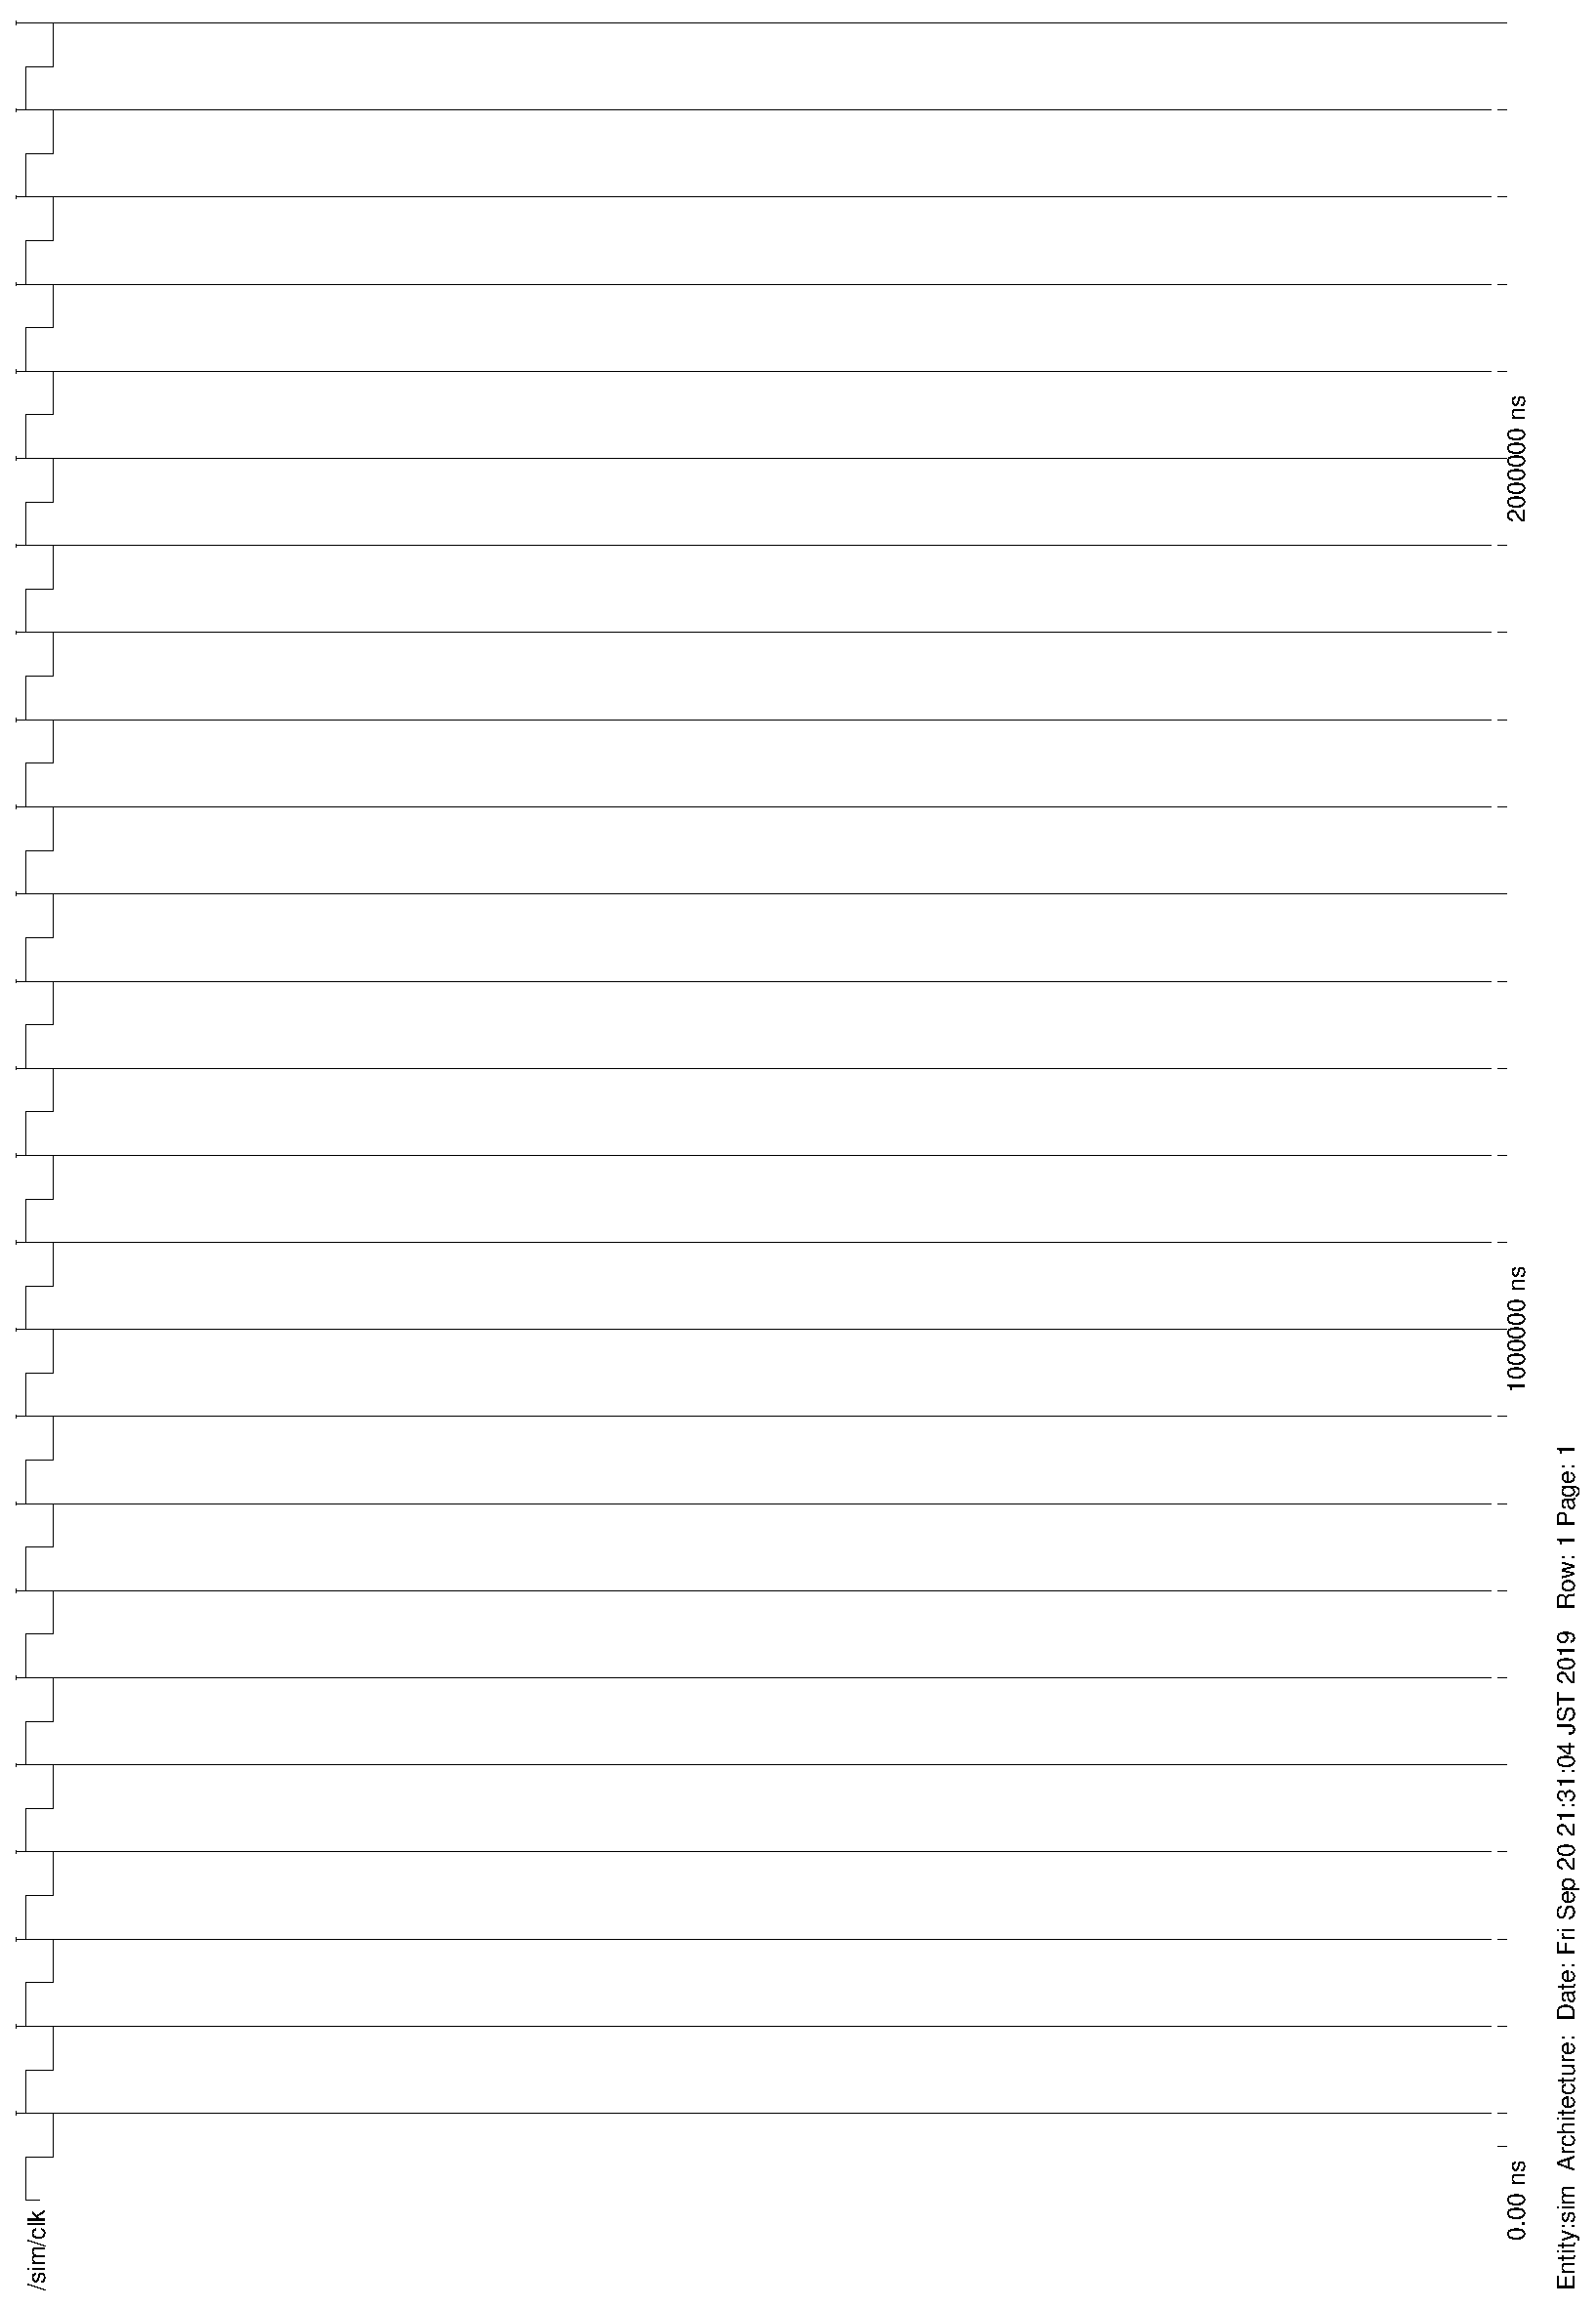
\includegraphics[height=\textheight]{wave-gate1.eps}\\[10mm]
        ゲートレベル記述のCPUの波形
    \end{center}
\end{figure}

\begin{figure}[p]
    \vspace*{-20mm}
    \begin{center}
        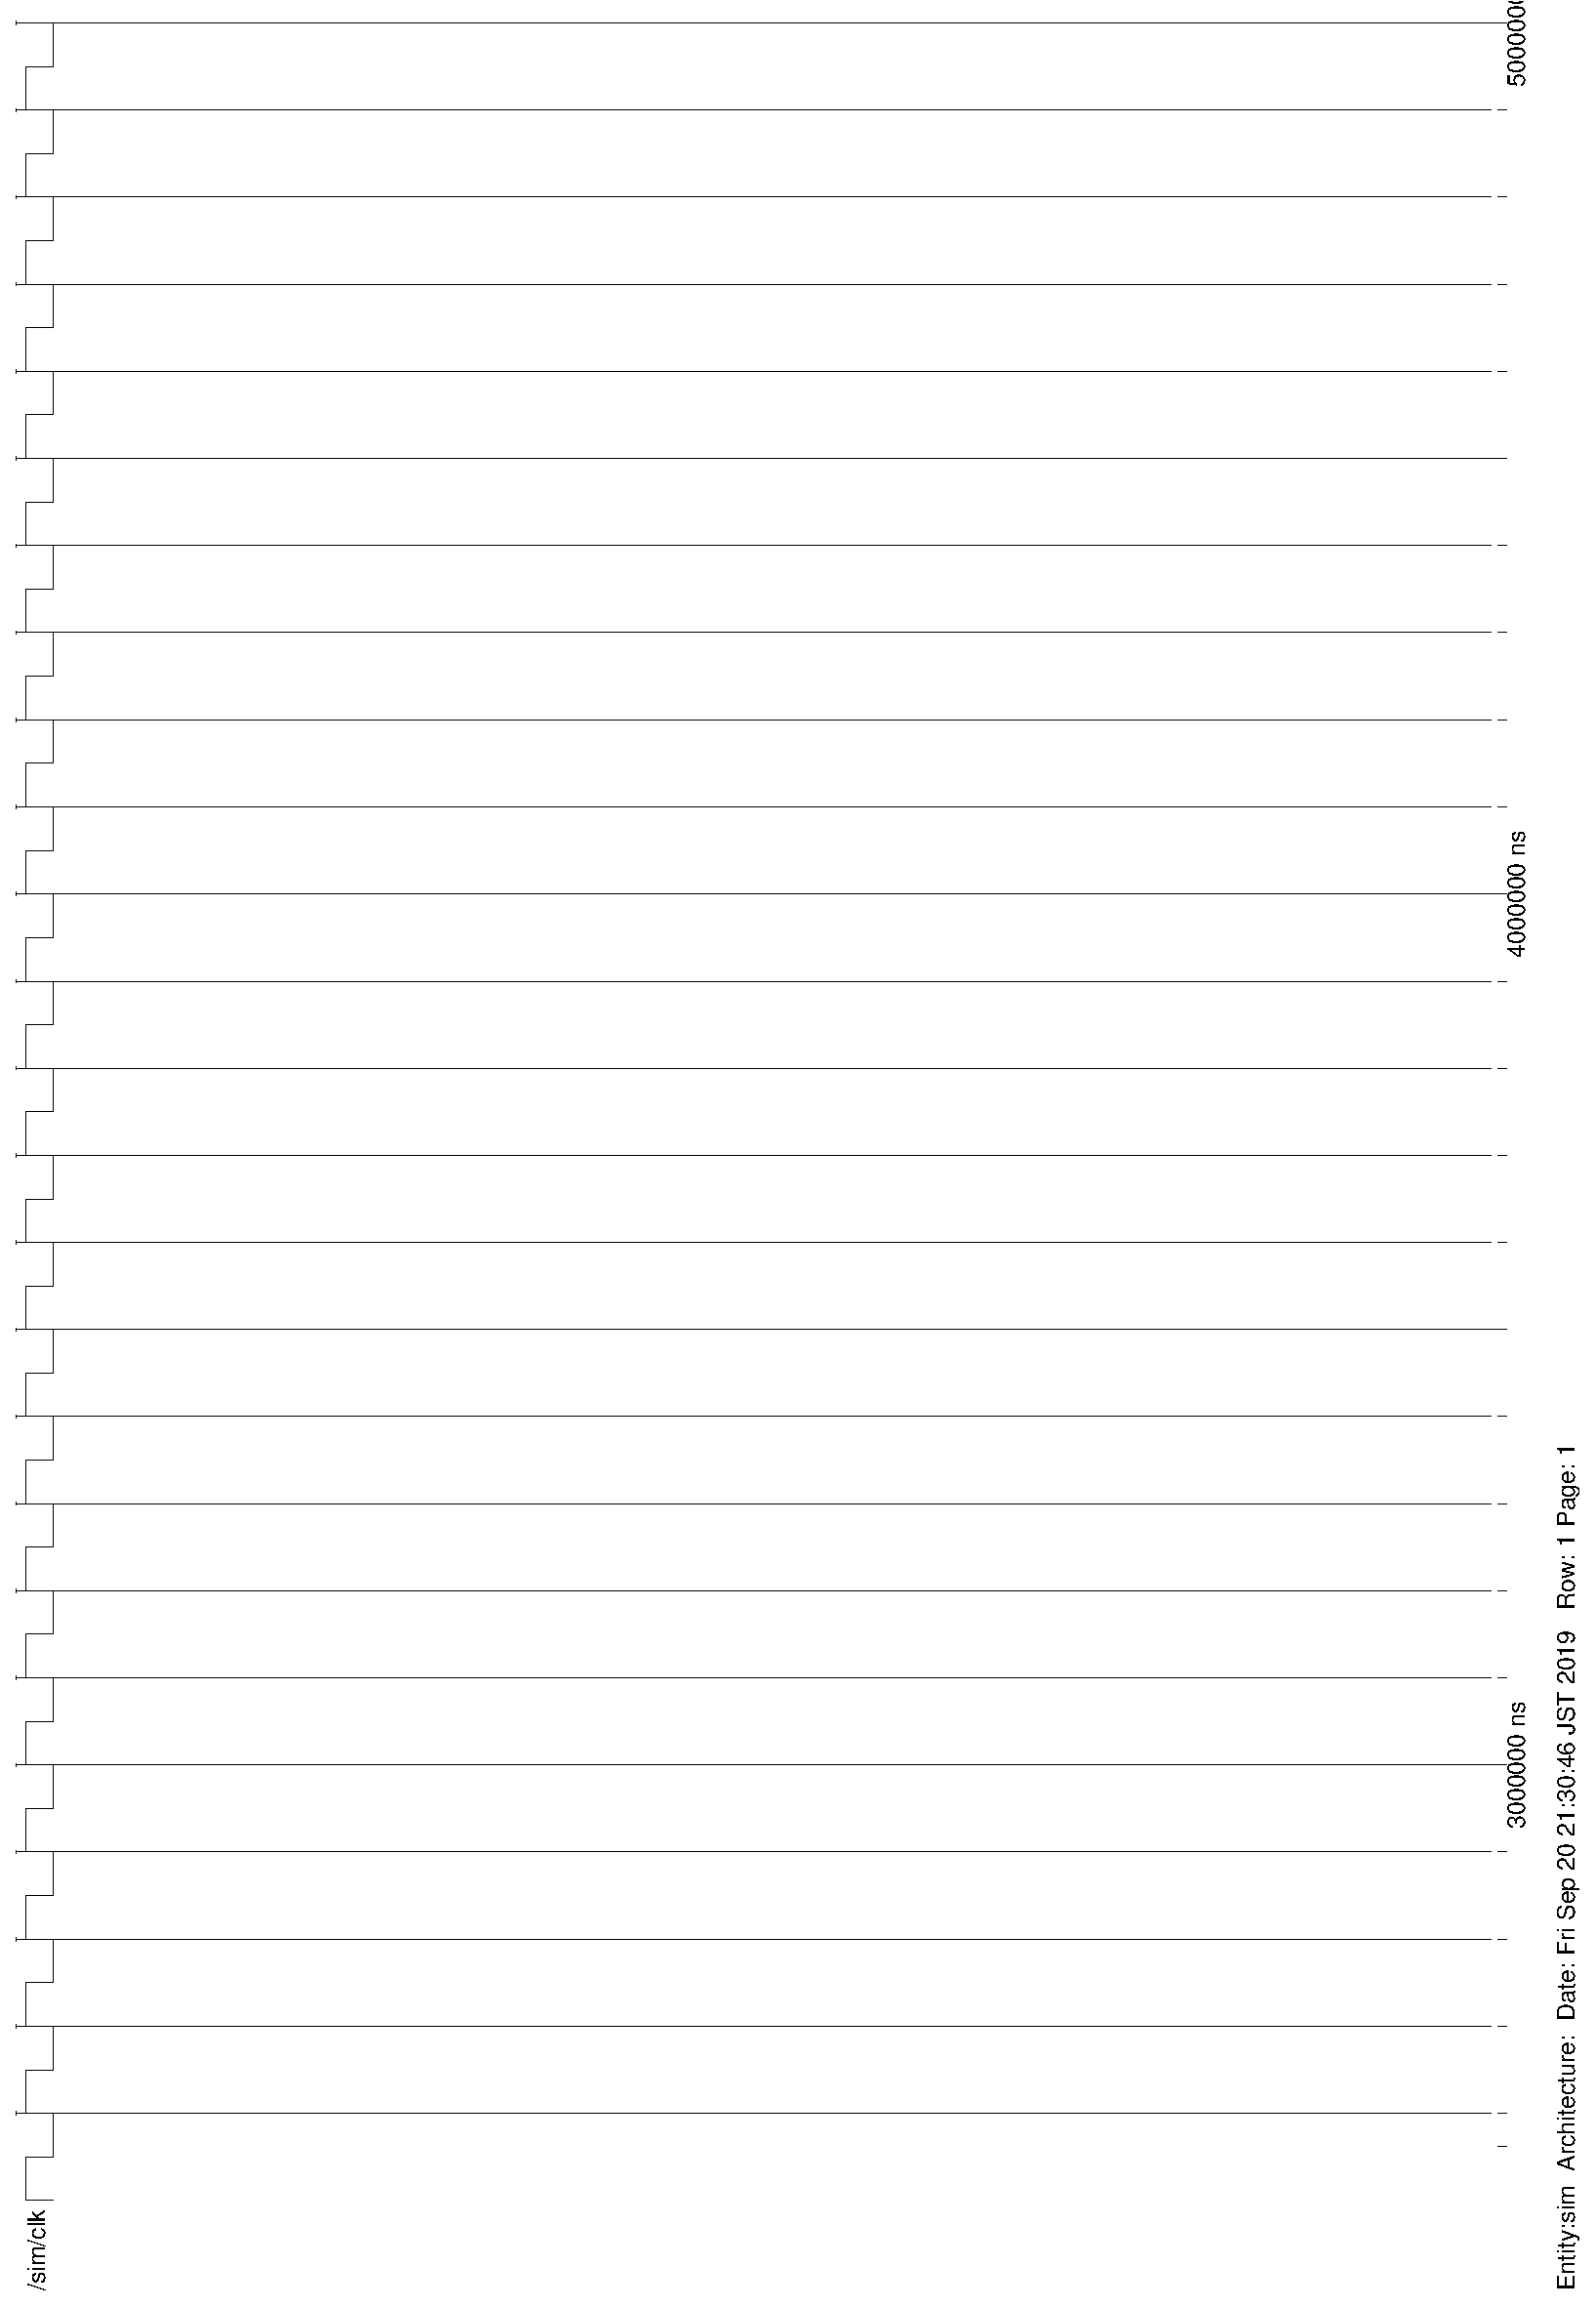
\includegraphics[height=\textheight]{wave-gate2.eps}\\[10mm]
        ゲートレベル記述のCPUの波形(続き)
    \end{center}
\end{figure}

\begin{figure}[p]
    \vspace*{-20mm}
    \begin{center}
        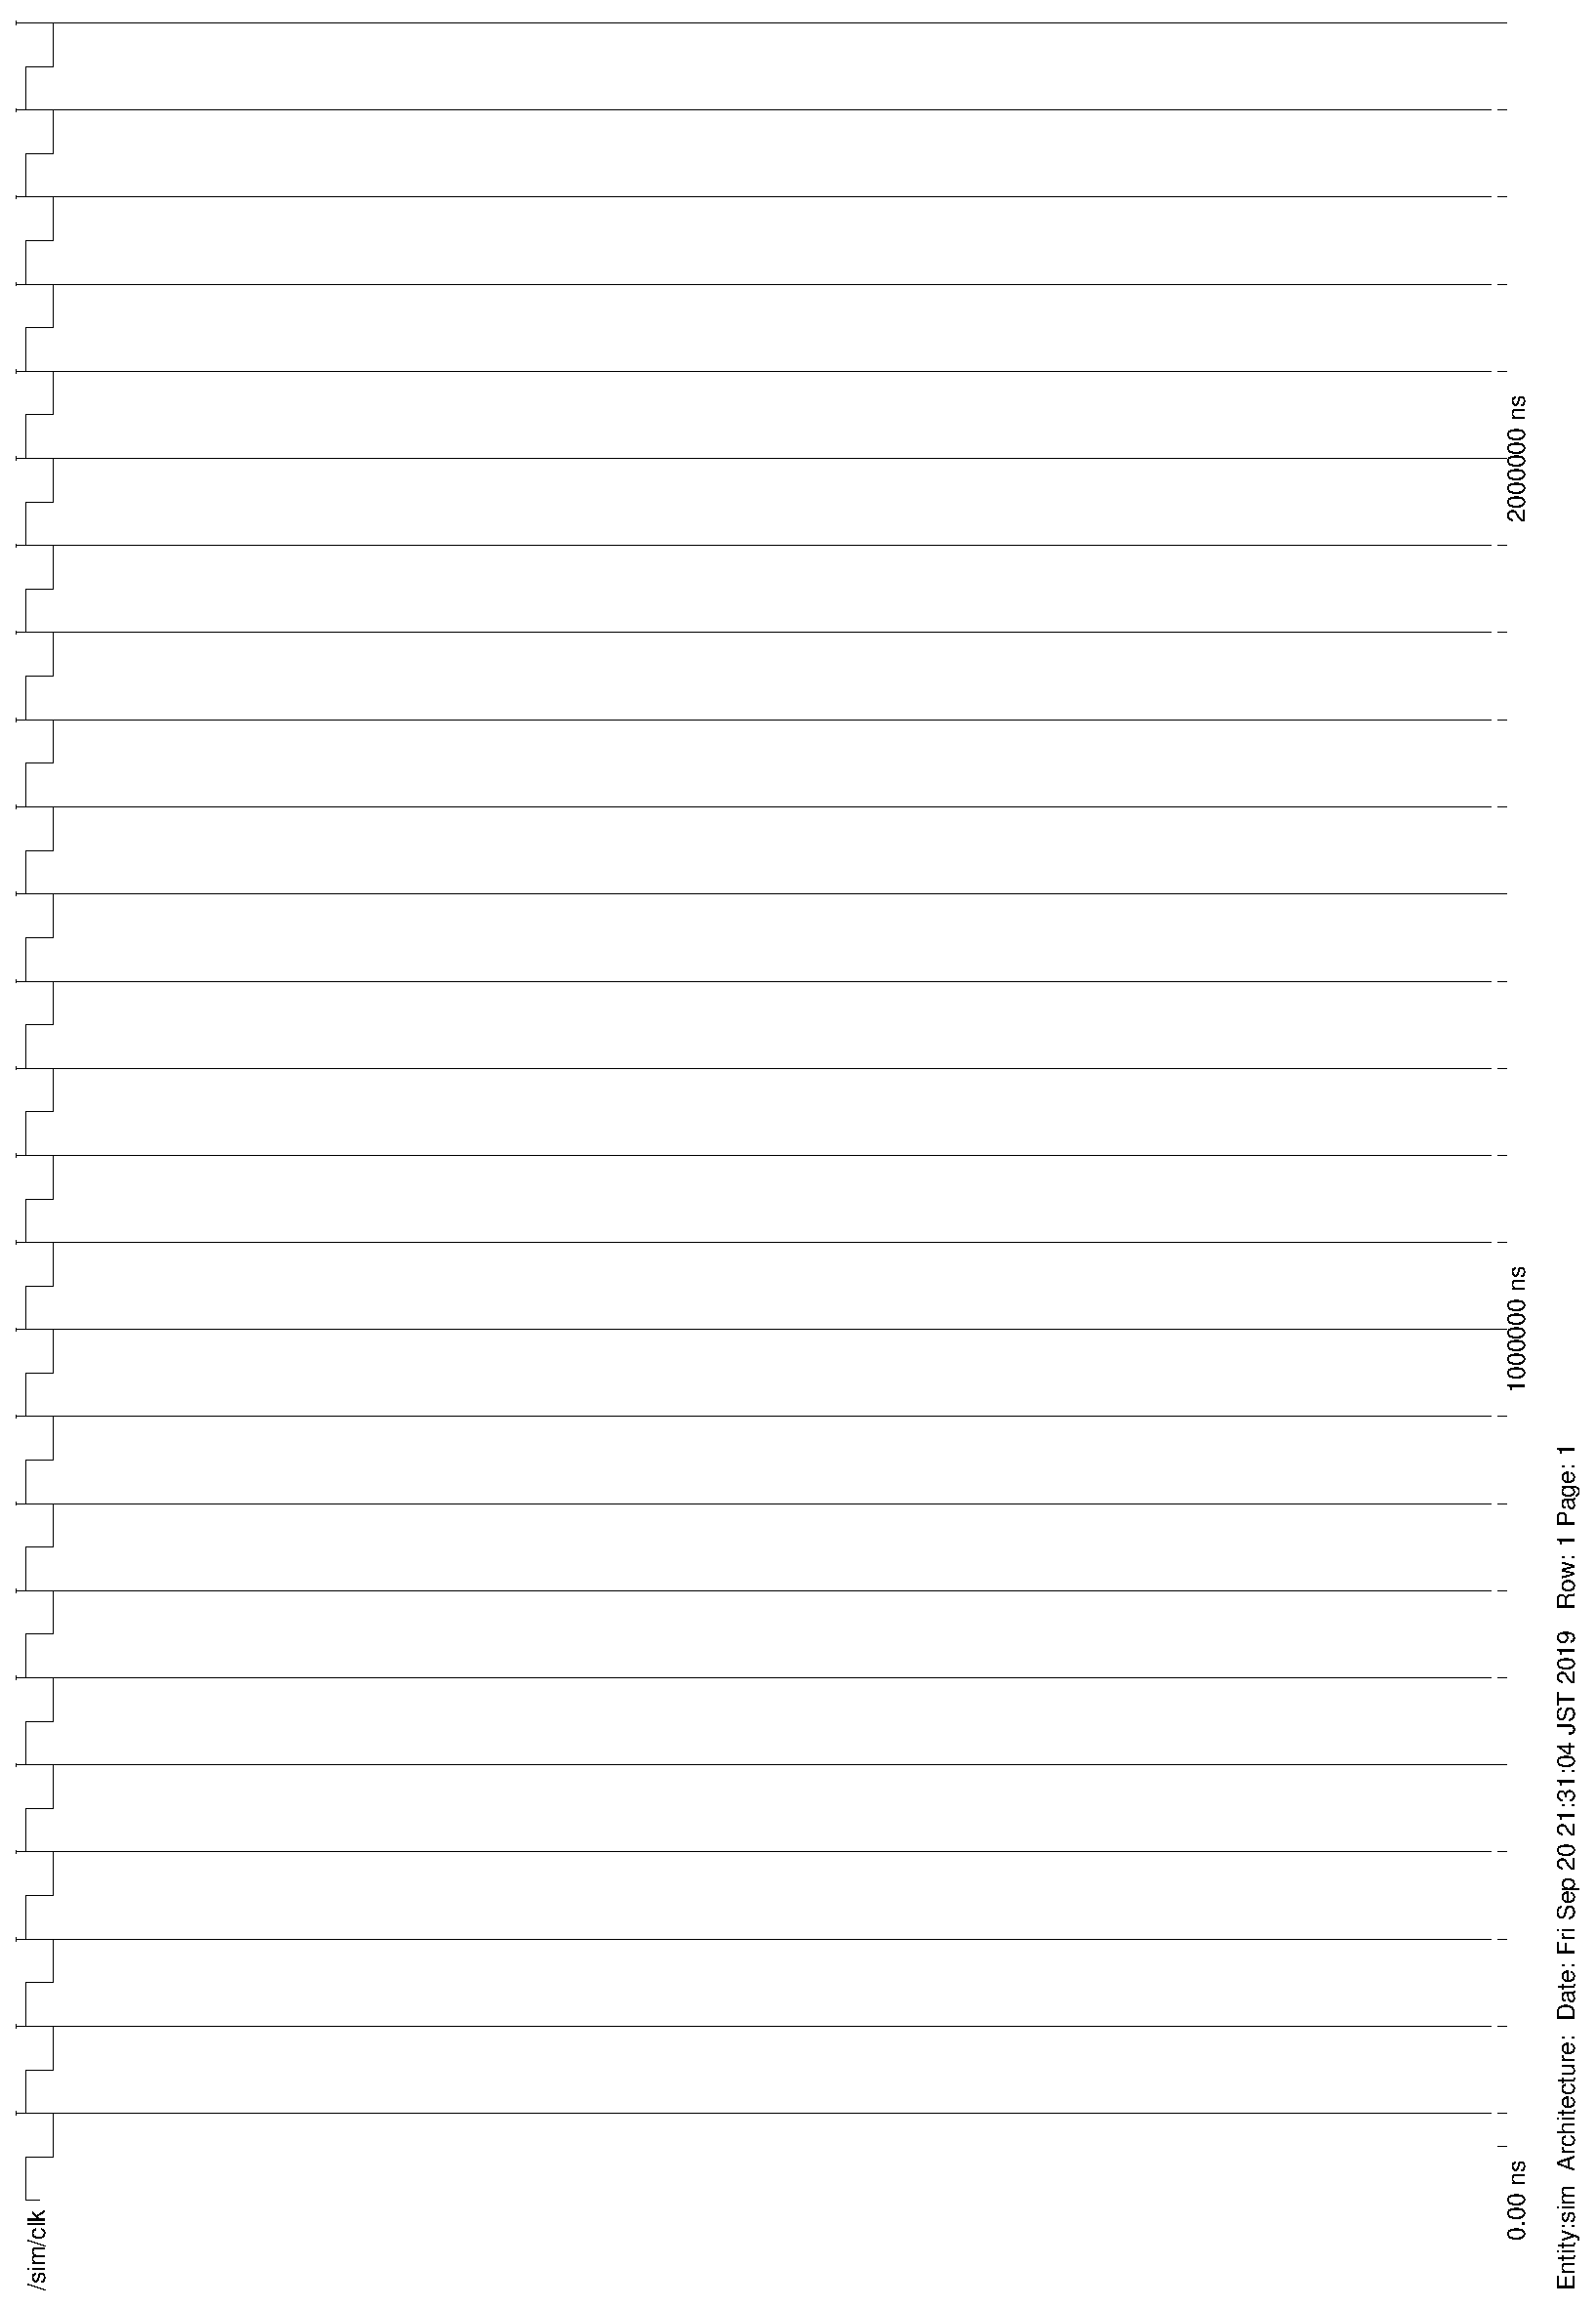
\includegraphics[height=\textheight]{wave-rtl1.eps}\\[10mm]
        RTL記述のCPUの波形
    \end{center}
\end{figure}

\begin{figure}[p]
    \vspace*{-20mm}
    \begin{center}
        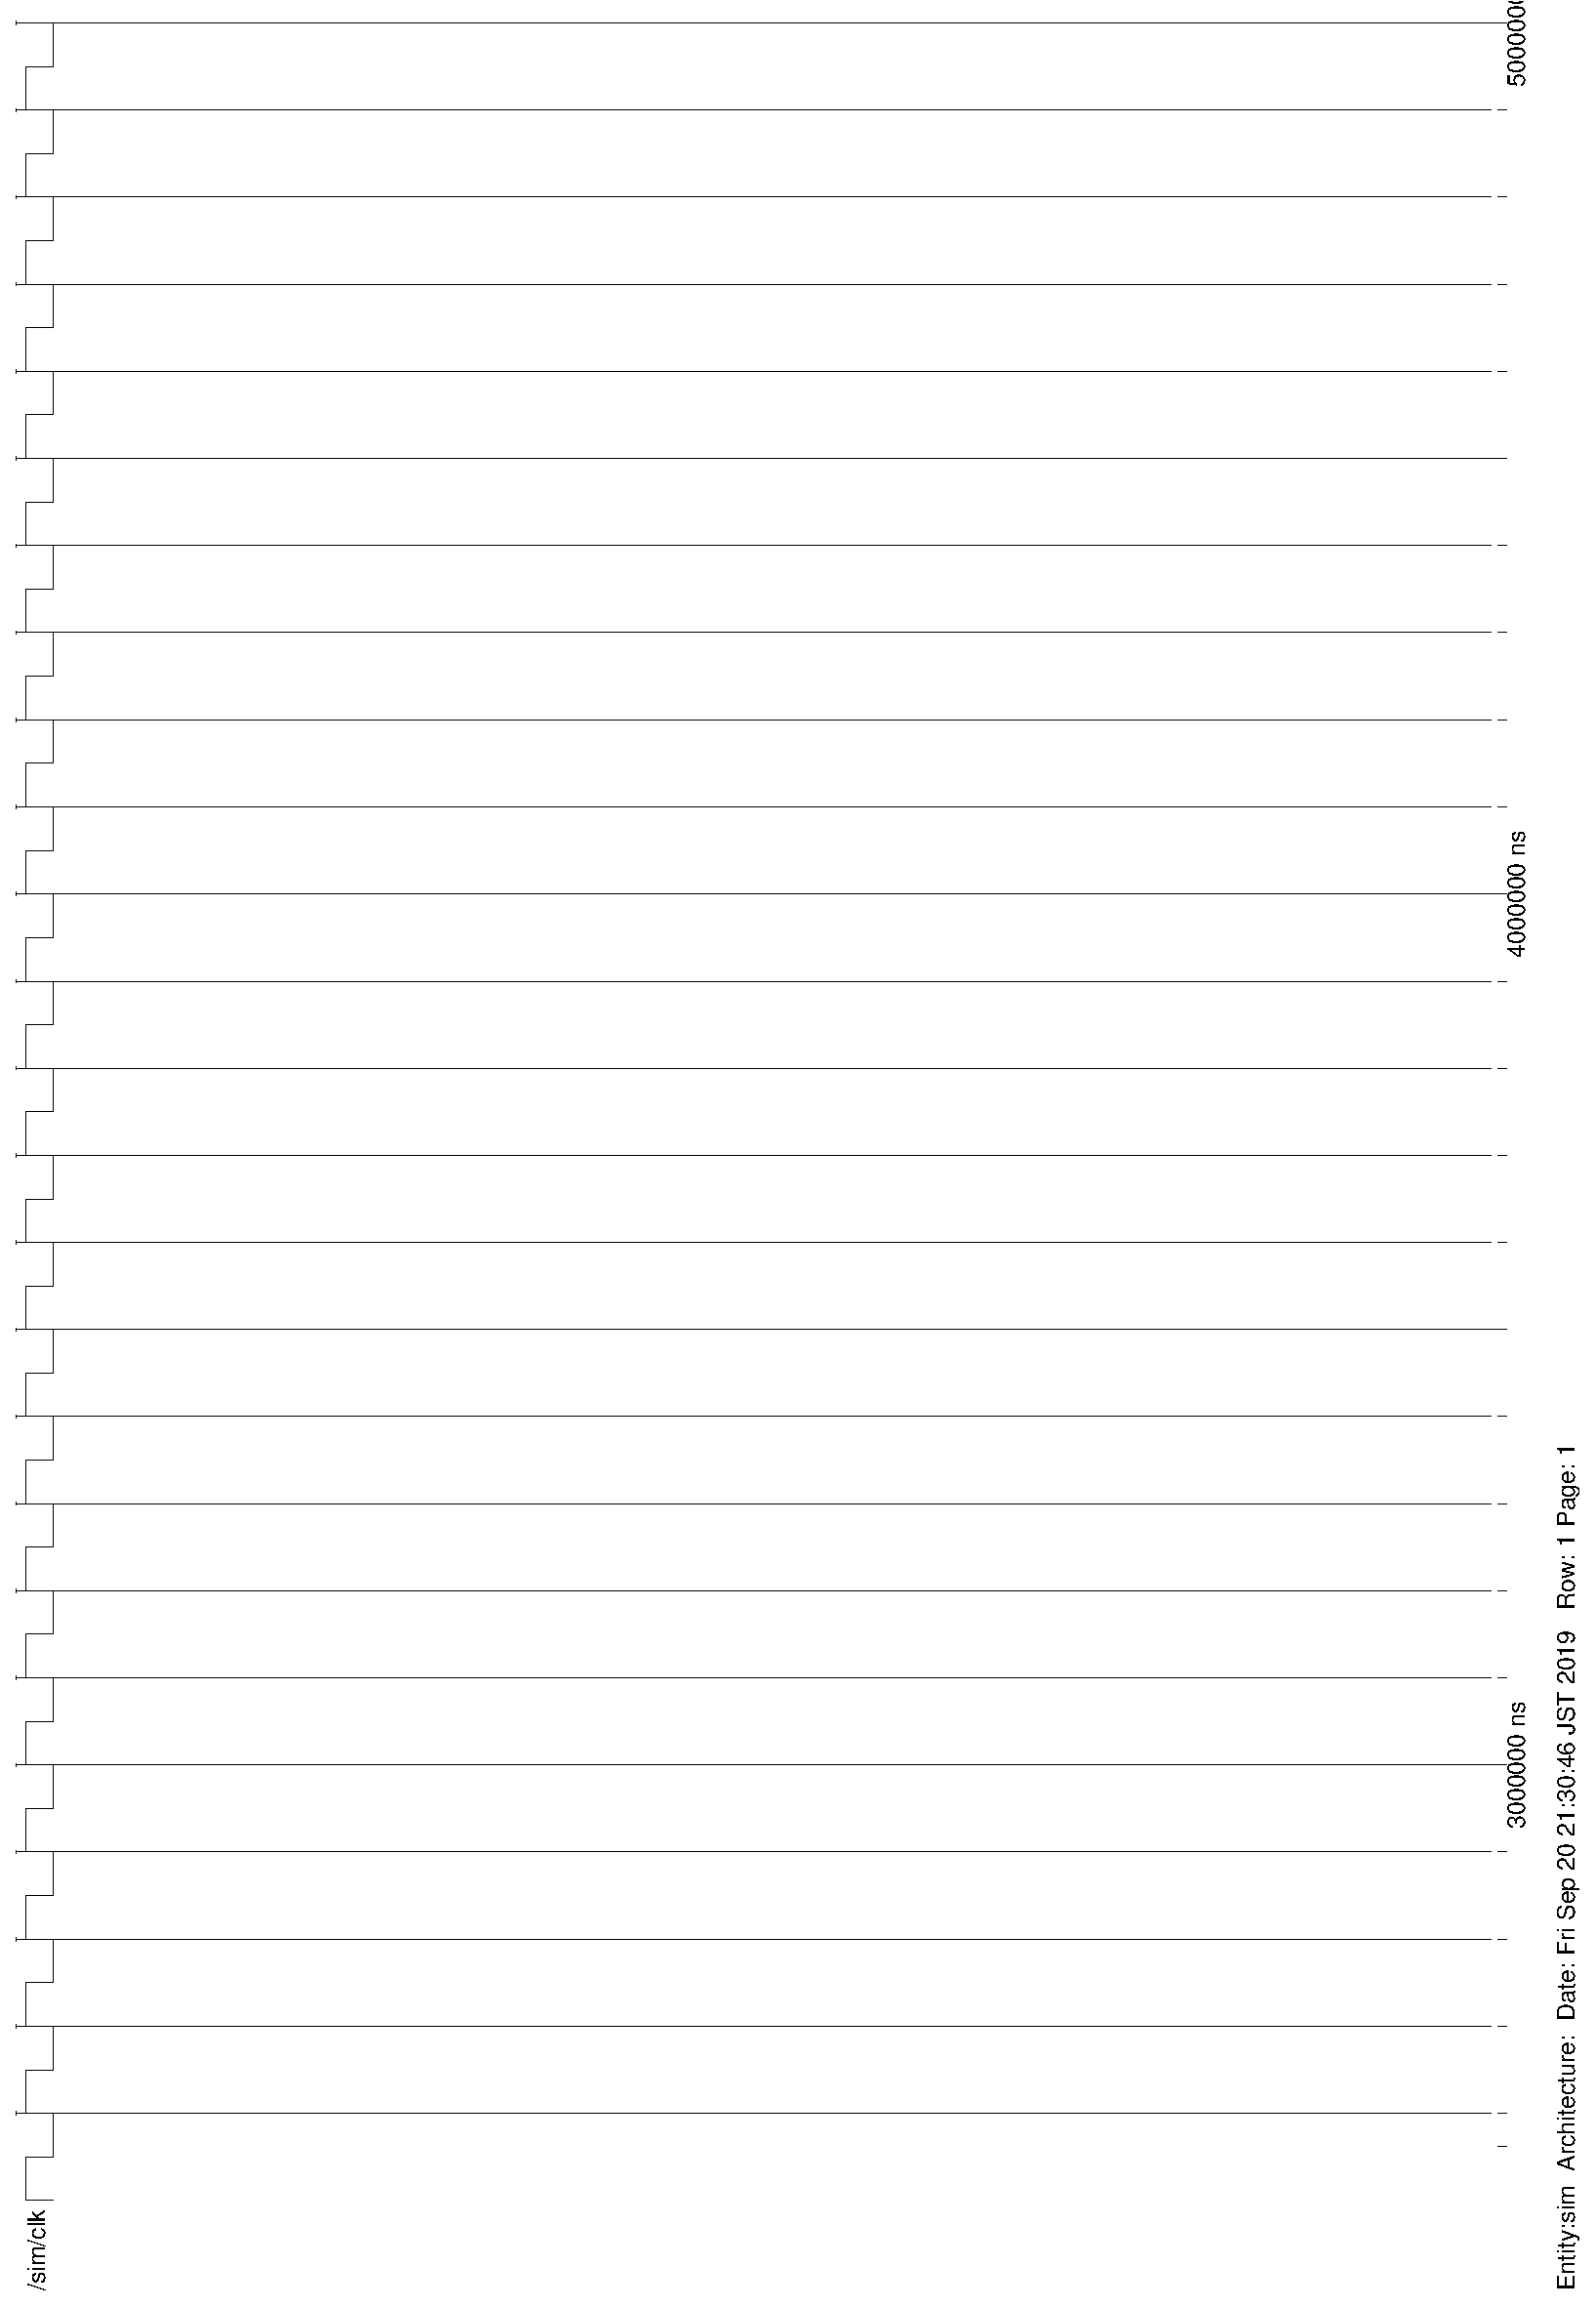
\includegraphics[height=\textheight]{wave-rtl2.eps}\\[10mm]
        RTL記述のCPUの波形(続き)
    \end{center}
\end{figure}

\end{document}
